\documentclass[11pt,letterpaper]{article}
\usepackage[hagavi]{azzam}

\title{Pelatda OSN SMP 2026 untuk DKI Jakarta}
\date{\today}
\begin{document}


% ============================================================
\section*{Algebra}
% ============================================================

\begin{enumerate}
    % Answer: 411/17  (Put a = cbrt(x-12), b = cbrt(3x-16), c = cbrt(2x-14). Cubing a + b = c gives (4x - 28) + 3abc = 2x - 14, so abc = (14 - 2x)/3; cubing again and writing w = 14 - 2x turns this into w[w^2/27 + (x-12)(3x-16)] = 0. The factor w gives x = 7, which checks out since cbrt(-5) + cbrt(5) = 0. The bracket gives 17x^2 - 292x + 1076 = 0 with positive discriminant 12096, and both roots -- about 11.8235 and 5.3535 -- satisfy the original equation, contributing 292/17. Total 7 + 292/17 = 411/17.)
    \item (OSN SMP 2022 \#3) Jumlah semua solusi real dari $\sqrt[3]{x - 12} + \sqrt[3]{3x - 16} = \sqrt[3]{2x - 14}$.

    % Answer: 4  (Dividing the two given relations gives R_n - R_{n+1} = a/k, a constant: the radius shrinks by the same amount every second. From V_1 = (27/64)V_0 we get (R_1/R_0)^3 = 27/64, so R_1 = (3/4)R_0 and the constant drop is R_0/4. Hence R_h = R_0 - h(R_0/4) = 0 at h = 4.)
    \item (OSN SMP 2015 \#10) Sebuah bola es memiliki volume awal $V_{0}.$ Setelah n detik (n bilangan asli), volume bola es menjadi $V_{n}$ dan luas permukaannya adalah $L_{n}$. Bola es mencair dengan perubahan volume per detik sebanding dengan luas permukaannya, yaitu $V_{n}-V_{n+1}=a~L_{n},$ untuk setiap n, dengan a adalah suatu konstanta positif. Selain itu, diketahui bahwa perbandingan antara perubahan volume dan perubahan jari-jari per detik sebanding dengan luas permukannya, yaitu $\frac{V_{n}-V_{n+1}}{R_{n}-R_{n+1}}=k~L_{n}$ dengan k adalah suatu konstanta positif. Jika $V_{1}=\frac{27}{64}V_{o}$ dan bola es mencair keseluruhannya tepat pada saat h detik, tentukan nilai h.

    % Answer: 4044  (Write the recurrence as 2a_{n+1}/a_n + 1 = sqrt(4a_n - 3) and square: 4(a_{n+1}^2 + a_n a_{n+1})/a_n^2 = 4a_n - 4, i.e. a_n^2 + a_n a_{n+1} + a_{n+1}^2 = a_n^3. So each summand is a_{i+1}^3/a_i^3, and from a_i^3 - a_{i+1}^3 = (a_i - a_{i+1})a_i^3 we get (a_{i+1}/a_i)^3 = 1 + a_{i+1} - a_i. Summing over i = 1..2021 telescopes to 2021 + (a_2022 - a_1). Since a_1 > 3 forces sqrt(4a_1 - 3) > 3, the sequence is increasing, so a_2022 - a_1 = 2023 and the sum is 2021 + 2023 = 4044.)
    \item (OSP SMA 2022 Isian Singkat \#10) Definisikan barisan $\{a_n\}$ dengan $a_1 > 3$ serta untuk semua $n > 1$, berlaku
    \[ 2a_{n+1}=a_n(-1+\sqrt{4a_n-3}) \]
    Jika $|a_1-a_{2022}|=2023$, nilai dari
    \[ \sum_{i=1}^{2021}\frac{a_{i+1}^3}{a_i^2+a_ia_{i+1}+a_{i+1}^2} \]
    adalah\dots

    % Answer: 2 + sqrt3 and 2 - sqrt3  (Let r = alpha^3 - 15alpha and s = alpha^4 - 56alpha. Then alpha^4 = alpha(15alpha + r) gives 15alpha^2 + (r-56)alpha - s = 0, so alpha is a quadratic irrational over the rationals. Substituting alpha^2 = ((56-r)alpha + s)/15 back into alpha^3 - 15alpha = r and killing the alpha-coefficient and the constant separately gives, with m = 56 - r, both s = 225 - m^2/15 and ms = 225(56 - m); eliminating s yields m^3 - 6750m + 189000 = 0, i.e. (m - 60)(m^2 + 60m - 3150) = 0. The quadratic factor has only irrational roots, so m = 60, r = -4, s = -15, and 15alpha^2 - 60alpha + 15 = 0 gives alpha^2 - 4alpha + 1 = 0.)
    \item (OSP SMA 2023 Esai \#4) Tentukan semua bilangan real takrasional $\alpha$ yang memenuhi
    \[ \alpha^3-15\alpha \quad \text{dan} \quad \alpha^4-56\alpha \]
    keduanya merupakan bilangan rasional.

    % Answer: ?  (belum dikerjakan -- nilai maksimum 3(a+b) di bawah kendala a+b+c = 8 dan ab+bc+ca = 0)
    \item (SMO Junior 2024) Let $a$, $b$ and $c$ be real numbers such that $a+b+c=8$ and $ab+bc+ca=0$. Find the maximum value of $3(a+b)$.
\end{enumerate}

% ============================================================
\section*{Number Theory}
% ============================================================

\begin{enumerate}[resume]
    % Answer: 611  (From a x b = 24 with a, b single digits the number aba is 383, 464, 646 or 838. If a Koleksi(n) has terms t_1, ..., t_j all greater than 1 with product n and sum s, the rest must be 1s, so the total number of terms is m = j + n - s: to maximise m, split n into as many prime factors as possible. For 383 (prime) m = 1; for 464 = 2^4 x 29, m = 5 + 464 - 37 = 432; for 838 = 2 x 419, m = 2 + 838 - 421 = 419; for 646 = 2 x 17 x 19, m = 3 + 646 - 38 = 611, the largest.)
    \item (OSN SMP 2021 \#8) Diketahui $aba$ adalah bilangan tiga digit dengan $a \times b = 24$. Koleksi($n$) adalah barisan bilangan bulat positif yang jumlah dan hasil kali semua sukunya sama dengan $n$. Sebagai ilustrasi, dua contoh Koleksi(12) adalah 1,1,1,1,2,6 dan 1,1,1,1,1,3,4. Jika $m$ adalah banyak suku dari Koleksi($aba$), tentukan nilai terbesar $m$ yang mungkin.

    % Answer: 6057  (Write X_(n) = X R_n with R_n = (10^n - 1)/9 the repunit. Since R_{2n} = R_n(10^n + 1), dividing by R_n turns the equation into A(10^n + 1) = 2B + C^2 R_n, i.e. 10^n(9A - C^2) = 18B - C^2 - 9A. The right side lies between -144 and 152 while 10^n >= 10, so both sides vanish: C^2 = 9A and 18B = C^2 + 9A = 18A, so B = A and A = k^2, C = 3k. With A, B, C in 1..9 this gives k = 1, 2, 3, that is (A,B,C) = (1,1,3), (4,4,6), (9,9,9). Each works for every n, so 3 x 2019 = 6057.)
    \item (OSN SMP 2019 \#10) $X_{(n)}$ melambangkan bilangan yang disusun oleh angka X sebanyak n. Sebagai contoh $2_{(3)}=222$, $5_{(2)}=55.$ Untuk A, $B,C\in\{1,2,3,...,9\}$ dan $1\le n\le2019$, tentukan banyaknya pasangan terurut (A, B, C, n) yang memenuhi $A_{(2n)}=2(B_{(n)})+(C_{(n)})^{2}$.

    % Answer: 78  (Put A = sqrt(2n-12) and B = sqrt(2n+40), so B^2 - A^2 = 52. If A + B = k is a positive integer then B - A = 52/k, so A = (k - 52/k)/2 and B = (k + 52/k)/2; these are integers only when k divides 52 and k and 52/k have the same parity. Among the divisors 1, 2, 4, 13, 26, 52 only k = 2 and k = 26 pass the parity test, and k = 2 gives A < 0. So k = 26, A = 12, B = 14, and 2n - 12 = 144 gives the single value n = 78.)
    \item (OSP SMA 2023 Isian Singkat \#7) Tentukan jumlah semua bilangan asli $n$ sehingga
    \[ \sqrt{2n-12}+\sqrt{2n+40} \]
    merupakan bilangan asli.

    % Answer: 15876  (Multiplying the six fractions makes every a_i cancel, leaving the product 1 x 2 x 3 x 4 x 5 x 6 = 720. Conversely, choosing any ordered 6-tuple of positive integers with product 720 for the six quotients determines the ratios a_1 : a_2 : ... : a_6 uniquely, and the gcd condition then pins down the tuple itself. So the answer is the number of ordered factorisations of 720 = 2^4 x 3^2 x 5 into 6 factors, distributing each prime's exponent independently: C(9,5) x C(7,5) x C(6,5) = 126 x 21 x 6 = 15876.)
    \item (JJMO Preliminary 2024 \#6) How many tuples of positive integers $(a_1,a_2,a_3,a_4,a_5,a_6)$ with greatest common divisor $1$ are there such that
    \[ \frac{a_1}{a_2},\ \frac{2a_2}{a_3},\ \frac{3a_3}{a_4},\ \frac{4a_4}{a_5},\ \frac{5a_5}{a_6},\ \frac{6a_6}{a_1} \]
    are all integers?

    % Answer: ?  (belum dikerjakan -- semua tripel (a,b,c) yang membuat ketiga ekspresi sekaligus berupa pangkat dua)
    \item (KTOM Juli 2023) Tentukan semua tripel bilangan asli $(a,b,c)$ sehingga ketiga bilangan berikut:
    \[ 2^a+2^b+3(c+1), \hspace{10pt} 2^b+2^c+3(a+1), \hspace{10pt} 2^c+2^a+3(b+1) \]
    semuanya adalah perpangkatan dua (dengan kata lain, dalam bentuk $2^k$ untuk suatu bilangan asli $k$).

    % Answer: ?  (belum dikerjakan -- bergantung pada palindrom enam digit mana yang merupakan hasil kali bilangan asli berurutan)
    \item (KTOM Juli 2023 Simulasi Pra OSN) Sebuah bilangan palindrom 6 digit dengan digit terakhir 4 merupakan hasil perkalian antara dua atau lebih bilangan asli berurutan. Hitunglah hasil penjumlahan digit-digit palindrom tersebut.

    % Answer: ?  (belum dikerjakan -- nilai x terkecil pada persamaan tersebut)
    \item (KTOM Juli 2023 Simulasi Pra OSN) Bilangan bulat positif $x$ dan $y$ memenuhi persamaan
    \[ x-y-\dfrac{x}{y}+\dfrac{x^5}{y^5}=2024. \]
    Tentukan nilai $x$ terkecil yang memenuhi.

    % Answer: ?  (belum dikerjakan -- semua n empat digit dengan f(n) = n)
    \item (SMO Open 2025) For any 4-digit positive integer $n$, define $f(n)=(a+b)^2$, where $a$ and $b$ are the numbers formed by the first two and the last two digits of $n$ respectively (leading zeros are allowed). For instance,
    \[ f(2025)=(20+25)^2=45^2=2025. \]
    Find all 4-digit positive integers $n$ such that $f(n)=n$.

    % Answer: ?  (belum dikerjakan -- bilangan 2024 digit terkecil yang membuat proses berhenti pada bilangan tetap)
    \item (EMC Junior 2024) Wiske wrote a 2024-digit positive integer on the blackboard. In each round of the game she erases the last digit of the integer, lets this digit be $d$, and writes down the sum of the remaining number and $2d$ in place of the old number. She repeats the same steps with the newly obtained number. After a certain number of rounds, Wiske found that the new number obtained was the same as the number in the last round, and she stopped the game. What is the smallest possible 2024-digit integer that Wiske started with in this game?

    % Answer: ?  (belum dikerjakan -- semua tripel bulat (a,b,c) pada persamaan tersebut)
    \item (North Korean MO 2014) Find all triples of integers $(a,b,c)$ such that
    \[ 5a^2+13b^2+c^2=a^2b^2. \]
\end{enumerate}

% ============================================================
\section*{Geometry}
% ============================================================

\begin{enumerate}[resume]
    % Answer: (sqrt6/9) pi a^3  (The solid is a regular octahedron; with edge s its volume is (sqrt2/3)s^3, so (sqrt2/3)s^3 = a^3 sqrt2 gives s^3 = 3a^3. The largest inscribed ball is the insphere, whose radius is s/sqrt6, so r^3 = s^3/(6 sqrt6) = a^3/(2 sqrt6) and the volume is (4/3) pi r^3 = 2 pi a^3/(3 sqrt6) = (sqrt6/9) pi a^3.)
    \item (OSN SMP 2019 \#8) Dua limas segiempat yang panjang seluruh rusuknya sama, alasnya berimpit membentuk suatu bangun ruang baru yang bernama bidang-8. Jika volume bidang-8 adalah $a^{3}\sqrt{2}$ cm$^{3}$, tentukan volume bola terbesar yang dapat dimuat oleh bidang-8 tersebut.

    % Answer: 116  (Place the intersection of the diagonals at the origin with AC on the x-axis and BD on the y-axis, so A = (-p,0), C = (q,0), B = (0,u), D = (0,-v) and P = (x,y); then Q = (x,0) and R = (0,y). Writing AQ = 5t, CQ = 3t, BR = 7w, DR = 2w gives AC = 8t, BD = 9w, so the area (1/2)(8t)(9w) = 36tw = 288 and tw = 8. Computing the two triangle areas by the shoelace formula and subtracting, everything except the following cancels: [ABP] - [CDP] = (1/2)[2w(p+q) - 5t(u+v)] = (1/2)(16tw - 45tw) = -29tw/2, whose absolute value is 29 x 8/2 = 116.)
    \item (OSP SMA 2025 Isian Singkat \#7) Diberikan segiempat konveks $ABCD$ dengan luas 288, $AC$ tegak lurus $BD$, dan $AB$ tidak sejajar $CD$. Misalkan $P$ suatu titik di dalam segiempat $ABCD$. Selanjutnya, misalkan $Q$ dan $R$ berturut-turut merupakan proyeksi titik $P$ pada sisi $AC$ dan $BD$. Jika $|AQ| : |CQ| = 5 : 3$ dan $|BR| : |DR| = 7 : 2$, maka selisih luas segitiga $ABP$ dengan luas segitiga $CDP$ adalah \dots
    Catatan: Segiempat konveks adalah segiempat yang memenuhi:
    \begin{itemize}
        \item Perpotongan kedua diagonalnya terletak didalam segiempat.
        \item Keempat sudut dalam dari segiempat tersebut kurang dari $180^\circ$.
    \end{itemize}

    % Answer: 23  (Since DP and EQ point the same way while DB and EC point opposite ways, the angle of EQ with EC is 180 degrees minus the angle of DP with DB. The sine rule in triangles BPD and EQC then gives BD = PB sin(angle BPD)/sin(angle PDB) and EC = QC sin(angle EQC)/sin(angle PDB); with angle BPD = angle EQC and BD = EC this forces QC = PB = 14. For the ratio, put B = (0,0), C = (3,0), D = (1,0), E = (2,0) and A = (x,y). Then P = 14A/19 and Q = (nA + mC)/(m+n) for AQ : QC = m : n, and the condition that DP is parallel to EQ reduces to -n = 14(m - 2n)/19, i.e. m : n = 9 : 14. Hence AQ = 9 and AC = 9 + 14 = 23.)
    \item (JJMO Preliminary 2026 \#6) In triangle $ABC$, two distinct points $D$ and $E$ lie on side $BC$ (excluding the endpoints) with $BD=DE=EC$. Points $P$ and $Q$ are taken on sides $AB$ and $AC$ (excluding the endpoints) so that line $DP$ is parallel to line $EQ$ and $\angle BPD=\angle EQC$. If $AP=5$ and $PB=14$, find the length of side $AC$. Here $XY$ denotes the length of segment $XY$.

    % Answer: sqrt41 - 3  (Take A as origin with b = AB and d = AD, so E = d + tb for some t in (0,1) and CE = (1-t)|b| = 3. Then M = (d + tb)/2, and intersecting line BM with AD gives F = d/(2-t), so DF = (1-t)|d|/(2-t) = 3. Writing u = (2-t)b, the conditions MB = |u - d|/2 = 5 and MC = |u + d|/2 = 4 give |u|^2 + |d|^2 = (100 + 64)/2 = 82. Now |u| = (2-t)|b| = 3(2-t)/(1-t) and |d| = 3(2-t)/(1-t) are equal, both equal to 3k with k = (2-t)/(1-t), so 18k^2 = 82 and k^2 = 41/9. Since k = 1 + 1/(1-t), AB = |b| = 3/(1-t) = 3(k-1) = sqrt41 - 3.)
    \item (JMO Preliminary 2026 \#6) Let $E$ be a point on side $CD$ (excluding the endpoints) of a parallelogram $ABCD$. Let $M$ be the midpoint of segment $AE$, and let $F$ be the intersection of line $BM$ with side $AD$. Suppose $CE=DF=3$. If $MB=5$ and $MC=4$, find the length of segment $AB$. Here $XY$ denotes the length of segment $XY$.

    % Answer: Terbukti  (belum dikerjakan -- soal pembuktian, EF = 3d/2)
    \item (Philippine MO 2026) Let $ABC$ be a triangle such that $AC-AB=BC-AC=d>0$. Let $\Omega$ be the circumcircle of $ABC$, let $D$ be the point on $\Omega$ which bisects the minor arc $AC$, and let $E$ be the foot of the altitude from $B$ to $AC$. The segment $BD$ meets $AC$ at a point $F$. Show that $EF=3d/2$.
\end{enumerate}

% ============================================================
\section*{Combinatorics}
% ============================================================

\begin{enumerate}[resume]
    % Answer: 112  (Let 5s be the total time of A, B, C together and 7u that of D and E, so 5s + 7u = 80 with every player on court for a positive time, hence s >= 3 and u >= 2. Reducing mod 5 forces u to be a multiple of 5, leaving u = 5 (then s = 9) since u = 0 is barred by u >= 2 and u = 10 would give s = 2 < 3. Writing 9 as an ordered sum of three positive parts gives C(8,2) = 28 ways and 5 as an ordered sum of two positive parts gives 4 ways, so 28 x 4 = 112.)
    \item (OSN SMP 2014 \#10) Pelatih tim nasional Bola Basket Indonesia akan memilih pemain untuk menjadi anggota tim inti. Pelatih akan menilai lima pemain A, B, C, D, dan E dalam satu pertandingan simulasi (atau uji coba) dengan total waktu pertandingan 80 menit. Setiap saat hanya ada satu di antara lima pemain tersebut yang bermain. Tidak ada pembatas banyaknya pergantian pemain selama pertandingan. Total waktu bermain untuk masing-masing pemain A, B, dan C adalah kelipatan 5 menit, sedangkan total waktu bermain masing-masing pemain D dan E adalah kelipatan 7 menit. Berapakah banyak cara setiap pemain berada di lapangan berdasarkan total waktu bermain?

    % % Answer: 191  (k = 19 and m = 1. Use the generating function f(x) = product of (1 + x^j) for j = 1..21 and the roots-of-unity filter, which counts the subsets with sum divisible by 4 as (f(1) + f(i) + f(-1) + f(-i))/4. The factor j = 1 makes f(-1) = 0, and each j congruent to 2 mod 4 contributes 1 + i^j = 0, so f(i) = f(-i) = 0 as well. Hence the count including the empty set is 2^21/4 = 2^19, and dropping the empty set leaves 2^19 - 1, so 10k + m = 190 + 1 = 191.)
    % \item (OSP SMA 2022 Isian Singkat \#9) Banyaknya himpunan bagian tak kosong dari $S \in \{1,2,\dots,21\}$ yang hasil penjumlahan anggotanya habis dibagi 4 adalah $2^k-m$ dimana $k$ dan $m$ bilangan bulat dan $0 \le m < 2022$. Nilai dari $10k+m$ adalah\dots

    % Answer: 68  (Over the two-letter alphabet {1,2}, three consecutive digits form 121 or 212 exactly when both consecutive pairs differ. So encode the string by its 7 "change / no change" steps: the forbidden patterns are precisely two consecutive changes. Binary strings of length 7 with no two adjacent 1s number F_9 = 34, and the first digit is free, giving 2 x 34 = 68.)
    \item (OSP SMA 2025 Isian Singkat \#6) Banyaknya bilangan asli 8 digit yang hanya terdiri dari digit-digit 1 atau 2 serta tidak memuat 121 maupun 212 adalah\dots
    Catatan:
    \begin{itemize}
        \item Contoh bilangan 5 digit yang memenuhi syarat tersebut adalah 12211 dan 22222.
        \item Contoh bilangan 5 digit yang tidak memenuhi syarat adalah 11211 dan 21222.
    \end{itemize}

    % Answer: 33  (Make the scores of ranks 1 to 99 equal to N, N-1, ..., N-98 and let rank 100 be M with rank 101 equal to M-1, everything below being tiny. Country J then scores s_1 + s_10 + s_100 = (2N - 9) + M. A rival with three of the remaining top-99 scorers totals about 3N and beats J easily, while a rival with two top scorers of ranks i, j plus the rank-101 participant beats J exactly when i + j < 10. Three disjoint such pairs exist -- (2,7), (3,6), (4,5) -- using six of the ranks 2..9; the 91 remaining high scorers (ranks 8, 9 and 11..99) then form 30 further countries. In total 3 + 30 = 33, and no arrangement does better.)
    \item (JJMO Preliminary 2023 \#7) In a competition entered by $100$ countries including Country $J$, a total of $300$ contestants --- three from each country --- take a test, and all of them obtain distinct non-negative integer scores. The contestants from Country $J$ obtain the $1$st, $10$th and $100$th highest scores among the $300$. Find the largest possible number of the remaining $99$ countries that satisfy the following condition:
    \begin{itemize}
        \item The sum of the scores of that country's $3$ contestants is greater than the sum of the scores of Country $J$'s $3$ contestants.
    \end{itemize}

    % Answer: ?  (belum dikerjakan -- peluang sebagai fungsi dari n)
    \item Choose $n$ points at random on a circle. What is the probability that all of the points lie in a semicircle?

    % Answer: Terbukti  (belum dikerjakan -- soal pembuktian keberadaan pewarnaan untuk setiap n >= 18)
    \item (Philippine MO 2017) Each of the numbers in the set $A=\{1,2,\dots,2017\}$ is coloured either red or white. Prove that for $n\ge 18$ there exists a colouring of the numbers in $A$ such that any of its $n$-term arithmetic sequences contains both colours.

    % Answer: ?  (belum dikerjakan -- nilai n mana yang dimenangkan Bob dan mana yang dimenangkan Alice)
    \item (Austrian MO Junior 2023) Alice and Bob play a game on a strip of $n\ge 3$ squares with two game pieces. At the beginning, Alice's piece is on the first square while Bob's piece is on the last square. The figure shows the starting position for a strip of $n=7$ squares.
    \begin{center}
    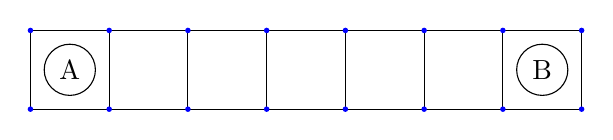
\begin{tikzpicture}
        % Draw the 1x7 grid
        \draw (0,0) grid (7,1);

        % Draw blue dots on the grid vertices
        \foreach \x in {0,...,7} {
            \foreach \y in {0,1} {
                \fill[blue] (\x,\y) circle (1pt);
            }
        }

        % Add the circled text nodes A and B
        \node[draw, circle, minimum size=6.5mm, inner sep=0pt] at (0.5,0.5) {A};
        \node[draw, circle, minimum size=6.5mm, inner sep=0pt] at (6.5,0.5) {B};
    \end{tikzpicture}
    \end{center}
    The players alternate. In each move, they advance their own game piece by one or two squares in the direction of the opponent's piece. The piece has to land on an empty square without jumping over the opponent's piece. Alice makes the first move with her own piece. If a player cannot move, they lose.
    \begin{itemize}
        \item For which $n$ can Bob ensure a win no matter how Alice plays?
        \item For which $n$ can Alice ensure a win no matter how Bob plays?
    \end{itemize}
\end{enumerate}

\end{document}
